\documentclass[border=8pt]{standalone}
\usepackage{tikz,amsmath,amssymb,bm}
\usetikzlibrary{arrows.meta,calc,angles,quotes,decorations.markings}
\begin{document}
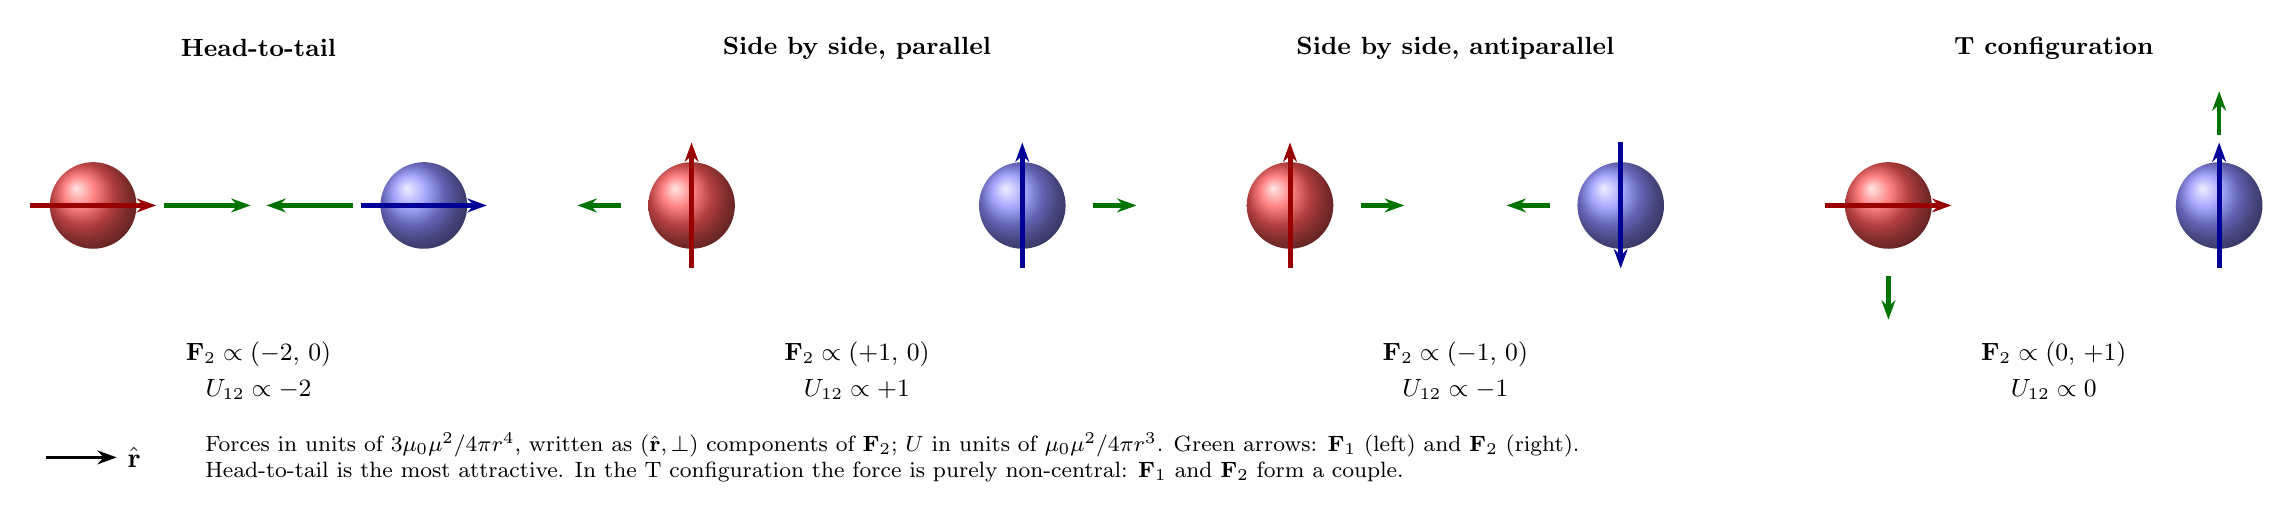
\begin{tikzpicture}[>={Stealth[length=7pt,width=5pt]},
  mom/.style={->,line width=1.8pt}, vec/.style={->,line width=1.1pt},
  aux/.style={densely dashed,gray!70},
  lbl/.style={fill=white,fill opacity=0.85,text opacity=1,inner sep=1pt,font=\footnotesize}]
\shade[ball color=red!65!white] (0.0000,0.0000) circle (0.55);
\shade[ball color=blue!45!white] (4.2000,0.0000) circle (0.55);
\draw[mom,red!60!black] (-0.8000,0.0000) -- ++(1.6000,0.0000);
\draw[mom,blue!60!black] (3.4000,0.0000) -- ++(1.6000,0.0000);
\draw[vec,green!45!black,line width=1.6pt] (3.3000,0.0000) -- ++(-1.1000,0.0000);
\draw[vec,green!45!black,line width=1.6pt] (0.9000,0.0000) -- ++(1.1000,-0.0000);
\node[font=\small\bfseries] at (2.1000,2.0000) {Head-to-tail};
\node[font=\small,align=center] at (2.1000,-2.1000) {$\mathbf F_2\propto(-2,\,0)$\\[2pt] $U_{12}\propto -2$};
\shade[ball color=red!65!white] (7.6000,0.0000) circle (0.55);
\shade[ball color=blue!45!white] (11.8000,0.0000) circle (0.55);
\draw[mom,red!60!black] (7.6000,-0.8000) -- ++(0.0000,1.6000);
\draw[mom,blue!60!black] (11.8000,-0.8000) -- ++(0.0000,1.6000);
\draw[vec,green!45!black,line width=1.6pt] (12.7000,0.0000) -- ++(0.5500,0.0000);
\draw[vec,green!45!black,line width=1.6pt] (6.7000,-0.0000) -- ++(-0.5500,-0.0000);
\node[font=\small\bfseries] at (9.7000,2.0000) {Side by side, parallel};
\node[font=\small,align=center] at (9.7000,-2.1000) {$\mathbf F_2\propto(+1,\,0)$\\[2pt] $U_{12}\propto +1$};
\shade[ball color=red!65!white] (15.2000,0.0000) circle (0.55);
\shade[ball color=blue!45!white] (19.4000,0.0000) circle (0.55);
\draw[mom,red!60!black] (15.2000,-0.8000) -- ++(0.0000,1.6000);
\draw[mom,blue!60!black] (19.4000,0.8000) -- ++(0.0000,-1.6000);
\draw[vec,green!45!black,line width=1.6pt] (18.5000,0.0000) -- ++(-0.5500,0.0000);
\draw[vec,green!45!black,line width=1.6pt] (16.1000,0.0000) -- ++(0.5500,-0.0000);
\node[font=\small\bfseries] at (17.3000,2.0000) {Side by side, antiparallel};
\node[font=\small,align=center] at (17.3000,-2.1000) {$\mathbf F_2\propto(-1,\,0)$\\[2pt] $U_{12}\propto -1$};
\shade[ball color=red!65!white] (22.8000,0.0000) circle (0.55);
\shade[ball color=blue!45!white] (27.0000,0.0000) circle (0.55);
\draw[mom,red!60!black] (22.0000,0.0000) -- ++(1.6000,0.0000);
\draw[mom,blue!60!black] (27.0000,-0.8000) -- ++(0.0000,1.6000);
\draw[vec,green!45!black,line width=1.6pt] (27.0000,0.9000) -- ++(-0.0000,0.5500);
\draw[vec,green!45!black,line width=1.6pt] (22.8000,-0.9000) -- ++(0.0000,-0.5500);
\node[font=\small\bfseries] at (24.9000,2.0000) {T configuration};
\node[font=\small,align=center] at (24.9000,-2.1000) {$\mathbf F_2\propto(0,\,+1)$\\[2pt] $U_{12}\propto 0$};

\draw[vec] (-0.6,-3.2) -- ++(0.9,0) node[right] {$\hat{\mathbf r}$};
\node[font=\footnotesize,align=left,anchor=west] at (1.3,-3.2) {%
 Forces in units of $3\mu_0\mu^2/4\pi r^4$, written as $(\hat{\mathbf r},\perp)$ components of $\mathbf F_2$; $U$ in units of $\mu_0\mu^2/4\pi r^3$.
 Green arrows: $\mathbf F_1$ (left) and $\mathbf F_2$ (right).\\
 Head-to-tail is the most attractive. In the T configuration the force is purely non-central: $\mathbf F_1$ and $\mathbf F_2$ form a couple.};
\end{tikzpicture}
\end{document}
